%\documentclass[sigconf, anonymous]{acmart}
\documentclass[conference]{IEEEtran}

%%\acmConference[ESEC/FSE 2020]{The 28th ACM Joint European Software %%Engineering Conference and Symposium on the Foundations of Software %%Engineering}{8 - 13 November, 2020}{Sacramento, California, United States}


% Fonte em português brasileiro
\usepackage[american]{babel}
\usepackage[utf8]{inputenc}
\usepackage{enumerate}
\usepackage{setspace}
\usepackage{pgfgantt}
\usepackage{booktabs}
\usepackage{listings}
\usepackage{hyperref}
\usepackage{xspace}
%\usepackage{balance}
% \usepackage[numbers]{natbib}
% \bibliographystyle{IEEEtranN}

% Default fixed font does not support bold face
\DeclareFixedFont{\ttb}{T1}{txtt}{bx}{n}{12} % for bold
\DeclareFixedFont{\ttm}{T1}{txtt}{m}{n}{12}  % for normal

% Custom colors
\definecolor{keywords}{rgb}{0.5,0,0.35}
\definecolor{comments}{RGB}{0,0,113}
\definecolor{red}{RGB}{160,0,0}
\definecolor{green}{RGB}{0,150,0}
 
\lstset{language=Python, 
        basicstyle=\ttfamily\small, 
        keywordstyle=\color{keywords}\bfseries,
        commentstyle=\color{comments},
        stringstyle=\color{red},
        showstringspaces=false,
        %identifierstyle=\color{red},
       }
       
% Identação e Margens
\usepackage{fullpage}      % Margens
\usepackage{indentfirst}   % Autoidentar

% Figuras
\usepackage{graphicx}       % Pictures

\title{On the Interplay Between Static and Dynamic Analysis for Mining Sandboxes}

 \author{
 %% \IEEEauthorblockN{Francisco Handrick da Costa}
 %% \IEEEauthorblockA{
 %% \textit{Computer Science Department} \\
 %% \textit{University of Brasília}\\
 %% Brasília, Brazil\\
 %% } \and
 %% \IEEEauthorblockN{Rodrigo Bonif\'{a}cio}
 %% \IEEEauthorblockA{
 %% \textit{Computer Science Department} \\
 %% \textit{University of Brasília}\\
 %% Brasília, Brazil\\
 %% }
}
%%\IEEEauthorblockA{
%%  \IEEEauthorrefmark{1}Computer Science Department, University of Bras\'{i}lia, Brazil}
%%  {francisco.tomaz@aluno.unb.br}
%%}
\begin{document}
\maketitle

\begin{abstract}
The popularization of Android platform and the growing number of Android apps that manage sensitive data, brought several security threats. Over the past years, researchers and practitioners have investigated techniques addressing Android's security issues, including techniques that leverage dynamic analysis to mine Android Sandboxes. Mining sandboxes through test generation tools is not a new strategy, and has been investigated before, however a potential combination with static analysis has not been sufficiently explored yet.

In this paper we investigate whether or not the use of static analysis might complement and increase the performance of dynamic analysis tools for mining Android sandboxes. Therefore, we first conducted a non-exact replication of a previous study \cite{DBLP:conf/wcre/BaoLL18} that compares dynamic test case generation tools for mining sandboxes, isolating all possible effects on the results of the static analysis tools the original work leverage to instrument the Android apps. We then conducted a new study to investigate the performance of tainted analysis algorithms for mining sandboxes.

Our results demonstrate that static analysis has an important contribution to the sandbox mining process, and its combination with dynamic analysis has the potential to improve malware detection techniques.


\end{abstract}

\begin{IEEEkeywords}
Malware Detection,
Mining Sandboxes,
Software Security,
Android Platform,
Empirical Studies,
Static Analysis and Dynamic Analysis
\end{IEEEkeywords}
\section{Introduction}\label{sec:introduction}

Almost two-thirds of the world use mobile technologies~\cite{Comscore}, and the Android Operating System has dominated the market of smartphones, tablets, and others electronic devices \cite{statcounter}. Due to this growing popularity, the number of incidents related to Android malicious software (malware) has significantly increased. In only three years, researchers reported a substantial increase in the population of Android malwares: from just three families and a hundred samples in 2010 to more than a hundred families with thousands of samples in 2013~\cite{DBLP:journals/comsur/FarukiBLGGCR15,DBLP:journals/csur/SufatrioTCT15}. Security issues in Android software applications~\footnote{In this paper, we will use the terms Android Applications, Android Apps and Apps interchangeably, to represent Android software applications} have become a relevant research topic, and many techniques have been developed to identify vulnerabilities in Android apps~\cite{DBLP:conf/pldi/ArztRFBBKTOM14}, including the use of static analysis algorithms either to identify privacy leaks or to reveal the misuse of cryptographic primitives~\cite{krueger:ecoop-2018,rahaman:ccs-2019}, for instance.

Another alternative for protecting users from Android malicious behavior consists in the use of dynamic analysis to mine Android sandboxes~\cite{DBLP:conf/icse/JamrozikSZ16}. The mine sandbox approach starts with an
exploratory phase, in which a practitioner takes advantage of automatic test case generator tools that explores an Android application while recording the set of sensitive APIs the app calls. 
. This set of senstivie calls comprises a sandbox infrastructure. After the exploratory phase, the sandbox might then monitor any call to sensitive APIs while a user is running the app, blocking the calls that have not been identified during the exploratory phase---thereby protecting Android users from additional malicious behavior~\cite{DBLP:conf/icse/JamrozikSZ16}.
Jamrozik et al. argue in favor of dynamic analysis for mining sandboxes, instead of using static analysis---mostly because of the overapproximation problem: ``static analysis often assume that more behaviors are possible than actually would be''~\cite{DBLP:conf/icse/JamrozikSZ16}. In addition, code that uses dynamic features (such as reflection) poses additional challenges to static analysis algorithms---even though \emph{dynamic features} of programming languages are often used to introduce malicious behavior. Even though these claims are reasonable, previous research results do not present empirical assessments about the limitations of static analysis to mine sandboxes. Consequently, it is not clear whether and how both approaches (dynamic and static analysis) could complement each other in the process of mining Android sandboxes.

The lack of understanding about static and dynamic analysis complementing each other also appears in the work of Bao et al.~\cite{DBLP:conf/wcre/BaoLL18} (hereafter \blls), which presents an empirical study that explores the performance of dynamic analysis for identifying malicious behavior using the mining sandbox approach.  %\kn{The use of word same here makes me wonder if readers could be confused. IMO the problem of how Static and dynamic analysis complement each other AND the role of static analysis in dynamic approaches are different (even if they sound similar), right? Reason I simply did not remove the word "same" is that I feel we need a bridge sentence here to make this transition of two similar sounding problems clear, because we only explore one of them.}
Their study leverages DroidFax~\cite{DBLP:conf/icsm/CaiR17a} to instrument $102$ pairs of Android apps (each pair comprising a benign and a malicious version of an App) and to collect the information needed to mine sandboxes (that is, the calls to sensitive APIs).
Although the authors report a precision of at most 70\% of dynamic analysis tools to differentiate the benign and malicious versions of the apps, the authors ignore the fact that DroidFax statically analyzes the Android apps and also records calls to sensitive APIs (besides instrumenting the apps). As we discuss in this paper, this DroidFax static analysis component leads to an overestimation of the performance of the dynamic analysis tools for mining sandboxes and might have introduced a possible threat to the conclusions of that work. {\color{red}In the security domain, overestimating the performance of a technique for malware identification brings serious risks, and we show here that DroidFax improves significantly the performance of the dynamic analysis tools for mining sandboxes.}

The goal of this paper is two fold. First we present the results of an
external, non-exact replication~\cite{role-of-replication} of the \blls. To this end,
we take advantage of DroidXP, a tool suite that helps researchers (including ourselves) to
integrate test case generation tools and compare their performance on
mining Android sandboxes. We discussed the design and implementation of DroidXP in a conference
paper~\cite{DBLP:conf/scam/CostaMCMVBC20}, which also
includes an initial evaluation of DroidXP.
As a matter of fact, the results of the first DroidXP evaluation revealed a possible
overestimation in the performance of dynamic analysis tools as
reported in the \blls---which in the end motivated us to
conduct the non-exact replication of that study. Here we extend
our previous work with a couple of customizations of DroidXP, which allowed us
to reproduce the \blls by means of a serie of new experiments
that reveal the actual performance of the
dynamic analysis tools. Section~\ref{sec:droidxp} revisit the
DroidXP design, while Section~\ref{sec:set1} discuss
the setup of our replication study.


%% In summary, our current study differs fromthe original work in three aspects: 

%% \begin{enumerate}[(a)]
%%   \item We isolate the effect of the static analysis component of DroidFax.
%%    \item We included a fake test
%% case generation tool (named \joke). \joke simulates a test tool that does not execute Android apps during DroidXP execution, disregarding the effects of dynamic analysis, and computing the results with only static analysis DroidFax component.
%% \item We extend the execution time and the number of executions of each test case generator tool for all apps
%% in our dataset.

%% \end{enumerate}
%% where offers direct access to all source code, installation process, dependencies, and how to run. We presented and evaluated DroidXP in a conference paper~\cite{DBLP:conf/scam/CostaMCMVBC20}, and here we discuss the results of a broader investigation that also uses DroidXP to explain the performance of static and dynamic analysis approaches for mining sandboxes. Our goal is to understand how static analysis algorithms might complement dynamic analysis approaches in the process of mining Android sandboxes. This work is an extension of SCAM 2020 paper, since that for our actual study, we had to adapt DroiXP to allow it to isolate the effects of static analysis component of DroidFax, and take into account this effect at our analysis.

%% Our research work presents the results of two empirical studies that aim to
%% address our research goal. In the
%% first study, we conduct a replication of the \blls, as presented at {\color{red}SCAN 2020} conference~\cite{DBLP:conf/scam/CostaMCMVBC20}, though 

Second, in this paper we also explore how a static analysis approach
(based on taint analysis) compares and complements the mining sandbox technique
for identifying malicious behavior that infects benign applications.
The idea here is to compare the dataflows from \emph{source} to
\emph{sink} statements computed using two executions of the
FlowDroid infrastructure~\cite{arzt:pldi-2014}: one execution that analyses
a benign version of an Android app and one execution that
analyses a malicious version. We consider that
the taint analysis approach is able to identify a malware whenever
we find a dataflow from a source to a sink in the second execution
that does not appear in the first one. We detail the
settings of this taint analysis study in Section~\ref{sec:set2}

Altogether, this paper brings the following contributions:

\begin{itemize}
\item A replication of the \blls that better clarifies the performance of
  dynamic analysis tools for mining Android sandboxes. The results of
  our replication (Section~\ref{sec:res-fs})
  give evidence that the previous work overestimated
  the performance of the dynamic analysis tools---that is, without
  DroidFax (an independent component used for running the
  \blls experiment), the performance of the tools drop between $16.44$\% to $58$\%. 

\item A broad comprehension about the role of static analysis tools for mining
  sandboxes, showing that we can benefit from using both static and dynamic
  analysis for detecting malicious Android apps. In addition,
  we give evidence that a well known static analysis approach, based on
  taint analysis, leads to a performance similar to the dynamic analysis
  approach for diferenciating benign and malicious versions of the same
  app (Section~\ref{sec:res-ss}).

\item A reproduction package of our study that is available online, including
  scripts for statistic analysis \footnote{https://htmlpreview.github.io/?https://github.com/droidxp/paper-replication-package/blob/master/replication.html}
  and tooling for reproducing and extending our study. The repository for DroidXP is available
at GitHub\footnote{https://github.com/droidxp/benchmark}.
 
\end{itemize}

\section{Background and Related Work}

%\kn{This section starts abrupt. We should have a line that says what concepts we introduce on a high level. Also, I feel "sandbox" itself should be one of the backgrounds and have a textbf after the introductory line.}

In this section, we introduce the concepts and terminology that are necessary to understand the remainder of this paper. First, Section~\ref{sec:sandbox} introduces some background information about the use of \emph{sandboxes} to protect invalid access to sensitive resources. After that, in Section~\ref{sec:android-sandbox} we review the mining sandbox approach for detecting malicious behavior in Android apps. Finally, Section~\ref{sec:taint} presents some background information about taint analysis.

\subsection{The Sandbox Approach for Protecting Resources}\label{sec:sandbox}

A \emph{sandbox} is an isolated environment on an electronic device within which applications cannot affect other programs outside its boundaries, like the file system, the network, or other device data~\cite{DBLP:journals/peerj-cs/MaassSCS16}. Sandboxes enable testing and execution of unsafe or untested code, possible malware, without worrying about the integrity of the electronic device that runs the application~\cite{DBLP:conf/esorics/BordoniCS17}. This need might arise in a variety of situations, such as when executing software input by untrusted users, in malware analysis, or even as a security mechanism in case a trusted system gets compromised~\cite{DBLP:journals/peerj-cs/MaassSCS16}.
A sandbox environment must be able to shield the host machine or operating system from any damages caused by third-party software. Thus, a sandbox environment should have the minimum requirements to run programs (make sure the program will not impact resources outside the sandbox), and make sure it will never assign the program greater privileges than it should have, working with the principle of \emph{least privilege}, giving permissions to users according to their needs, i.e., giving them no more power than needed to successfully perform their task. This principle prevents escalating privileges and unauthorized access to resources, thereby improving the system's overall reliability.

Within the Android ecosystem, least privilege is realized through sandboxing process, where apps never access the data of other apps, and an app just accesses user resources, like contacts and location, through specific APIs (Application Programming Interface), which are in-turn guarded by permissions. Google Play Store is the primary market source for Android apps, and has a flexible policy regarding the apps' publishment process. Therefore, every month administrators remove several Android apps from the Play Store because of issues related to spyware and other types of malware \cite{DBLP:conf/msr/WangLL0X18}. For security reasons, Google Play lists each app with its requested permissions. However, many malicious apps usually ask for more permissions than their APIs normally would require~\cite{DBLP:conf/ccs/FeltCHSW11}. Those permissions are presented to the user during a new app's installation, since Android version 6, but most users are careless since they are only interested in the end product~\cite{DBLP:conf/soups/FeltHEHCW12}. 

Nowadays, malware becomes more stealthy and hackers learn how to avoid anti-virus signature checks, for instance by obfuscating calls to native code that is allowed to make system calls~\cite{DBLP:journals/corr/abs-2002-04540} or conducting side attacks to make system calls from a benign app.

\subsection{Mining Android Sandbox}\label{sec:android-sandbox}

The mining Android sandbox approach~\cite{DBLP:conf/icse/JamrozikSZ16} relies on test generator tools to explore an Android app's dynamic behavior, and thus mine a set of sensitive resources the app needs. The sandbox uses this set of sensitive APIs to ensure the app execution's security by restricting the resources that are allowed to use. The mining sandbox approach works in two phases. In the first, named exploratory phase, a practitioner uses test generator tools to execute a benign version of an app and record the set of sensitive APIs the app calls. In the second phase, named execution, the sandbox constraints the app to access only the sensitive APIs mined in the first phase. Accordingly, the sandbox ensures that a malicious app could not call any sensitive API, besides those calls to APIs recorded in the first phase.

The idea of automatically mining software resources or components to infer behavior is not new, and has been discussed before. For instance, Whaley et al.~\cite{DBLP:conf/issta/WhaleyML02} combine dynamic and static analysis for API mining and so infer program behavior based on an usage example of Java classes. Ammons et al.~\cite{DBLP:conf/popl/AmmonsBL02} propose a machine learning approach, called specification mining, to discover temporal and data-dependence relationships that a program follows when interacting with an API or abstract data types.

The main purpose of a test generator tool is to program crashes or bugs in general. Nonetheless, it is also possible to use test generator tools to explore program behavior (dynamic analysis), and thus assist in the task of building sandboxes. Regarding test generator tools used for mining Android sandboxes, Jamrozik et al~\cite{DBLP:conf/icse/JamrozikZ16} proposed DroidMate, a test generation tool that implements a pseudo-random graphical user interface (GUI) exploration strategy, and was the first approach to leverage test generation to extract sandbox rules from apps. Li et al.~\cite{DBLP:conf/icse/LiYGC17} proposed DroidBot, a test generator tool that explores sensitive resources access from Android apps, following a model-based exploration strategy. In their work, the authors present a comparison between DroidBot and Monkey~\cite{Monkey} regarding malware analysis and show that DroidBot can trigger several sensitive calls more often than Monkey. Sensitive calls in the Android context occurs when an Android app functionality can result in accessing or leaking of Android users' sensitive data. Examples of sensitive calls access user location or network information. Humanoid is another test generator tool for Android~\cite{DBLP:conf/kbse/LiY0C19}---actually a DroidBot evolution. It is also a GUI test generator that learning how humans interact with Android apps. In contrary to random input generators, Humanoid uses a learned model to generate human-like test inputs, and prioritize the possible interactions on a GUI, according to their importance.


Bao et al.~\cite{DBLP:conf/wcre/BaoLL18} present a comparative study test generator tools to identify malicious behavior using the mining sandboxes approach. Their study indicates that the tools were efficient in identifying at most $70$\% of the malware in a specific dataset and also reports that after, combining all test generator tools, it was possible to detect $75.49$\% of malicious behavior explored ($77$ among $102$). However, this study did not focus on the possible interference of static analysis in the final result, since this study used DroidFax~\cite{DBLP:conf/icsm/CaiR17a} to instrument the apps, though, as we discuss in this paper, DroidFax also performs a static analysis of the apps whose results complement the dynamic analysis approach for mining sandboxes.

\subsection{Taint Analysis}\label{sec:taint}

Taint analysis is a special type of static or dynamic analysis that aims to track data flows within programs~\cite{DBLP:conf/sigsoft/PauckBW18}. Typically, taint analysis is used to identify sensitive information leakage by detecting taint flow between ``sources'' and ``sinks''. In the context of Android apps, a data leak occurs when sensitive data, such as contact, or device ID, flows from a sensitive resource to a method that might \emph{sink} information to other peers, like sending a message. Taint analysis can present possible malicious data flow to malware detection tools or even for a human check, which can decide if the ``source-sink" relationship is or is not an unwanted behavior. Thereby, taint analysis monitors sensitive sources ``tainted" through the app by starting at a pre-defined point. 

In the Android context, sources are the APIs in which apps access sensitive information, called sensitive APIs. The analysis follows the data flow until it reaches a sink, like a method that sends SMS. It brings precise information about which data will be leaked~\cite{DBLP:conf/pldi/ArztRFBBKTOM14}. The Android SDK provides APIs that allow apps to send private data to other apps on the same device, or remote devices. As these APIs may lead to sensitive data leakage, they are security-critical and require special attention and control~\cite{DBLP:conf/osdi/EnckGCCJMS10}. (Listing~\ref{lst:sourceSink}) presents a simple data leakage example. In this example, the device information is captured at line 4 (source) and then leaked at line 9 (sink), by SMS transmission.


\begin{lstlisting}[caption={Simple Data Leakage},
      language=Java, basicstyle=\fontsize{8}{6}\selectfont\ttfamily,
      label={lst:sourceSink}]

1 > localObject2 = (TelephonyManager)getSystemService("phone");
2 > if (localObject2 != null)
3 > {
4 >  this.imei = ((TelephonyManager)localObject2).getDeviceId();//source
5 > }
6 > if ("".equals(this.destMobile)) {
7 >  getDestMobile();
8 > }
9 > sendSMS(this.destMobile, "imei:" + this.imei)//sink
\end{lstlisting}


Wei et al.~\cite{DBLP:conf/issta/HuangDMD15} propose a scalable taint analysis for Android apps that applies traditional taint analysis techniques with targeted optimizations specific to Android OS. FlowDroid~\cite{DBLP:conf/pldi/ArztRFBBKTOM14} improves the precision of traditional approaches by including context and flow sensitivity. A significant issue with taint analysis is the cost of the tool itself hampering the performance. FastDroid~\cite{DBLP:journals/compsec/ZhangTD21} mitigates this issue by introducing an intermediate light-weight abstraction to perform the analysis, called taint value graph (TVG). To improve efficiency and precision, FastDroid focuses on exploring the propagation of taint values, rather than the traditional data flow analysis. FastDroid constructs taint value graphs (TVGs) exploring taint values, then it extracts a subset of potential taint flows (PTFs) from it. FastDroid improves the analysis process by performing analysis only on (PTFs). In this paper we investigate the use of taint analysis to identify malicious behavior, by mining the source an sink pairs from distinct versions of an app.

\section{Malware characterization}
\section{Study Settings}

%\kn{This paragraph requires a motivation. The details of Boa's study must be described upfront. Something like "Boa et al.'s study performs ..... Since their study also involved a static analysis component whose impact was not measured, we perform a non-exact replication to understand the impact static analysis may have had in the results...}


In this section
we present the settings of our study, whose goal is to build a general understanding of the implications of using static analysis algorithms
to complement a dynamic analysis approach
for mining Android sandboxes. % We also investigate how static analysis can improve the performance of mining sandboxes, in the task of identifying malicious behavior.
To achieve this goal, we answer the following research questions.

\begin{enumerate}[(RQ1)]
 
 \item What is the impact of the DroidFax static analysis algorithms into the results of the \blls?
  
 \item What is the effective performance of each test generation tool, in terms of the number of detected malware, when we
   discard the contributions of the DroidFax static analysis algorithms?

 \item What are the benefits of using taint
 analysis algorithms to complement the dynamic analysis approach for mining sandboxes?
\end{enumerate}

%\kn{Droidfax comes out of nowhere. We should introduce this or if already introduced earlier, remind the readers of where it stands with the Bao study in the first line of this section when describing boas study}

Answering the research questions RQ1 and RQ2 allows us to expose a possible overestimation in terms of the number of detected malware by each sandbox, constructed by the test
generation tools explored in \blls. Ignoring the implications of DroidFax in the \blls might have introduced a possible threat to their conclusions. Answering research question RQ3
allows us to open up the possibility of finding new strategies for malware detection, complementing the performance of
dynamic analysis through the use of static analysis algorithms.
We conducted two studies to answer the research questions above. In the
first study we leverage DroidXP~\cite{DBLP:conf/scam/CostaMCMVBC20} (Section~\ref{sec:droidxp}) to replicate
the \blls. We present the settings of this first study in Section~\ref{sec:set1}.
In the second study we use
FlowDroid~\cite{DBLP:conf/pldi/ArztRFBBKTOM14} to investigate the 
suitability of taint analysis algorithms to complement mining Android sandboxes. The main idea of this second study is explore the possibility of detected extra malware, do not detected at our first study, through another static analysis strategy based on taint analysis. We present the settings of the second study in Section~\ref{sec:set2}. 


\subsection{The DroidXP benchmark}\label{sec:droidxp}

We used DroidXP to systematically assess and compare the performance of test generation tools for mining android sandboxes. DroidXP relies on a
simple \emph{Command Line Interface} (CLI) that simplifies the integration of different test generation tools and favors the setup and execution 
of the experiments. DroidXP also relies on DroidFax, which instruments Android apps and collects relevant information about
their execution, including the set of sensitive APIs a given
app calls during a test execution. DroidFax also collects inter-component communication (ICC) using  static
program analysis.


The DroidXP CLI provides commands for listing all test case
generation tools (executing the project with the option ``list-tools'') that had been
integrated into the benchmark and commands that execute the experiments. An
experiment run can be configured according to several parameters, including:

\begin{itemize}
    \item \texttt{-tools}: Specifies the test tools used in the experiment
    \item \texttt{-t}: Specifies the threshold (in seconds) for the execution time in the experiment
    \item \texttt{-r}: Specifies the number of repetitions used in the experiment
    \item \texttt{-output-format}: Specifies the output format
    \item \texttt{--debug}: Specifies to run in DEBUG mode (default: false)
    \item \texttt{--disable-static-analysis}: Disable DroidFax static analysis phase (default: false)
\end{itemize}

Figure~\ref{fig:benchArq} shows the DroidXP architecture, based on the pipes-and-filters architectural style \cite{architecture-book}. 
The architecture includes three main components; where each component is responsible for a specific phase of the
benchmark (instrumentation, execution, and result analysis).

\begin{figure*}[thb]
  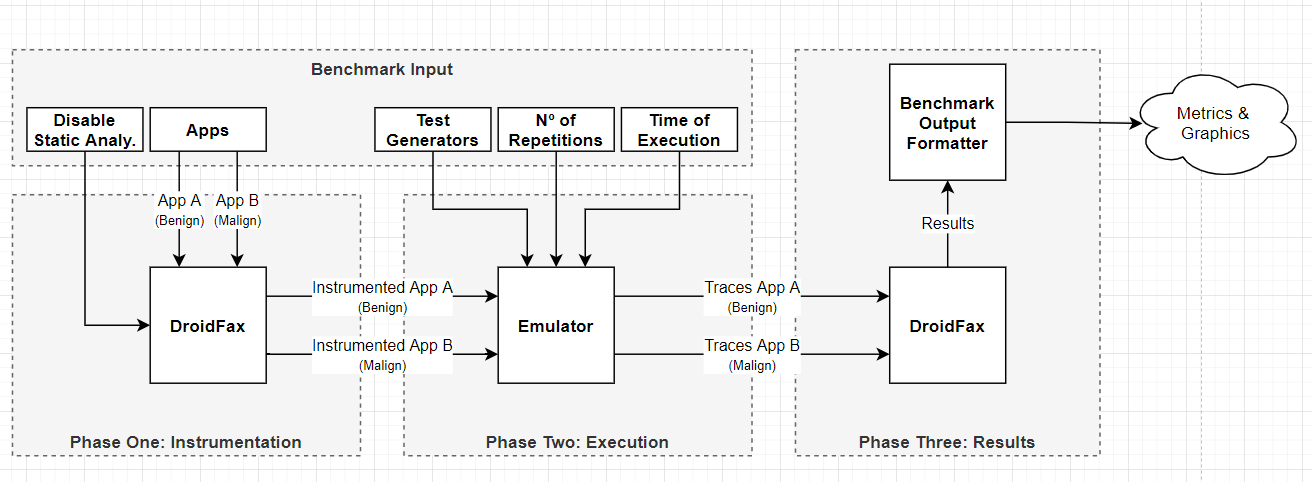
\includegraphics[width=1\textwidth]{images/benchmark4.png}
  \label{benchArq}
  \caption{Benchmark architecture}
  \label{fig:benchArq}
\end{figure*}
\subsubsection{Phase 1: Instrumentation}

In the first phase, a researcher must define the corpus of APK files DroidXP should consider during a benchmark execution. After that, DroidXP starts the DroidFax service that instruments each APK file, so that DroidXP would be able to collect data about each execution. To improve the performance of the benchmark, the instrumentation phase runs only once for each APK. In this phase, the DroidFax tool also runs some static analysis procedures---when the option \texttt{--disable-static-analysis} is not set.

\subsubsection{Phase 2: Execution}

In this phase, DroidXP installs an (already instrumented) APK file into
an Android emulator, and then executes a test case generation tool
during a period of time. This process repeats for every test case generation
tool and APK files. To provide repeatability of the experiment, DroidXP removes all data stored in the emulator before starting
a new execution. That is, every execution uses a \emph{fresh} emulator,
without any information that might have been kept during
previous executions. 

It is relatively easy to add new test
case generation tools into DroidXP. To achieve this goal, it leverages the Strategy Design
pattern~\cite{patterns-book}, which sets a contract between a family of classes that, in our case, abstracts the particularities
for running each tool we want to integrate into DroidXP.
%To carry out our replication study, we successfully integrated all
%test generation tools previously mentioned into DroidXP: Monkey, DroidBot, DroidMate, and
%Humanoid. 

\subsubsection{Phase 3: Result Analysis}

During the execution of the instrumented apps, all data that is relevant to our
research is collected by Logcat~\cite{Logcat}, one of the Android SDK's native tools. Logcat dumps a log from the Android emulator
while the already instrumented app is in execution. The part of the log we analyze in this phase comprises
the data sent by the methods within the Android app that were instrumented on the first
phase using the DroidFax tool. 

This data includes method coverage from the execution of each test generator tool and the
set of sensitive APIs the app calls during its execution. This set of calls to
sensitive APIs is necessary to estimate the test generator performance in identifying malicious apps---by spotting
differences between the sensitive API accessed by each version of an app (benign or malign).
In the end, the benchmark outputs the results of the experiment, which gives the
performance of one or more testing generator tools in mining sandboxes.

We used the DroidXP infrastructure to conduct the replication of
the \blls, whose settings we present in the following section. 

\subsection{First Study: A replication of the \blls}\label{sec:set1}

The \blls reports the results of an empirical study that compares the performance of test generation tools to mine Android
sandboxes. Since the \blls does not
compute the possible impact of DroidFax into the performance of the test generation tools,
here we replicate their work to understand the impact of the DroidFax static analysis algorithms into the \blls results.

Our replication differs from the original work in a few decisions. First, here we isolate
the effect of the DroidFax static analysis algorithms, in the task to identify malicious apps. In addition, although we use the same dataset of
$102$ pairs of Android apps used in the \blls, here we discarded $6$ pairs for which
we were not able to instrument---out of the $102$ pairs used in the original work, originally shared in the AndroZoo repository~\cite{DBLP:conf/msr/AllixBKT16}. We also introduced a recent test generator tool (Humanoid ~\cite{DBLP:conf/kbse/LiY0C19}), which
has not been considered in the previous work. Finally, we extended the execution time of each test generation tool,
executing each app from the test generation tool for three minutes (instead of one minute in the
original work),
and built the sandboxes after executing each test generation tool
three times---the original work executed each test generation tool
only once. That is, our goal here is not to conduct an
exact replication of the \blls, but instead understand
the role of the DroidFax static analysis algorithms in the
performance of test case generation tools for mining sandboxes.
% The original study executed each app at each tool, for just one minute, and just one time.

Besides Humanoid, our study considers three test generation tools used in the \blls: DroidBot~\cite{DBLP:conf/icse/LiYGC17},
DroidMate~\cite{DBLP:conf/icse/JamrozikZ16}, and Monkey~\cite{Monkey}. We selected DroidBot and DroiMate because they achieved
the best performance on detecting malicious behavior---when considering the $102$ pairs of Android apps (B/M) in the \blls.
It is important to note that here we used a new version of DroidMate (DroidMate-2), since it presents several enhancements
in comparison to the previous version. We also considered the Google's Monkey open source tool, mostly because it is the most
widely used test generation tool for Android~\cite{DBLP:conf/sigsoft/ZengLZXDLYX16}. Monkey is part of the Android SDK
and does not require any additional installation effort. We included Humanoid in our study
because it is a recent tool that emulates realistic users, creating human-like test inputs using deep learning techniques.

\subsubsection{Sensitive APIs extraction process}


In our first study, sensitive APIs extraction process starts with monitoring of invocations of sensitive APIs during the apps (already instrumented) execution by test generation tools under analysis. This task is essential for the process since sensitive APIs are used to access resource sensitives and it call could be a clue of private data leakage. Our study based at a list of 97 sensitive APIs, defined by the AppGuard privacy-control framework~\cite{DBLP:conf/esorics/BackesGHMS13}. Initially, we performances the extraction process using the default settings of DroidXP, (e.g., using DroidFax static analysis component). We explored the four test case generation tools described earlier and a fake test case generation tool (named \joke). 

\joke simulates a test tool that does not execute the Android apps during the exploratory phase. Using this tool the results of the dynamic analysis are not considered, and we can compute the results with only the static analysis component of DroidFax (RQ1). Our study executed each 96 pair of
Android app (B/M) in each test generation tool, including \joke, for three minutes, and for three times.

Then we repeated this process, however this time we used a DroidXP configuration that disables the DroidFax static analysis algorithm.
With this new configuration, we monitored sensitive APIs invocations again, using the same 96 pair of Android app (B/M), the same execution time,
and the same test case generation tools. With this new configuration, became possible computer the effective performance of each test generation tool, in terms of malware detected, discarding the contributions of DroidFax static analysis algorithm (RQ2). 

\subsubsection{Sensitive APIs analysis procedures}

After exploring all sensitive APIs by all test tools, we analyzed the \emph{performance} of these tools to detect malicious behaviors. The procedure starts with the analysis of each sandbox modeled by their respective test generation tools, based on the calls to sensitive APIs.

The test generation tool \emph{performance} is measured as the total number of malware, your respective sandbox is able to identify when comparing the calls to sensitive APIs made by the benign and malign versions of the app. We raise a warning (a \emph{hit}) whenever a sandbox finds that the malicious version of an app calls additional sensitive APIs, in comparison to the calls from the corresponding benign version. Figure \ref{fig:setup} shows all the phases of our experiments, that explore all sensitive resources access by both apps (B/M), and the optional configuration DroidXP, which disables DroidFax static analysis.

Assuming that our fake test case generation tool does not run the Android apps, its \emph{performance} analysis will reveal the DroidFax static algorithms impact at \blls, answering our first research question (RQ1). The analysis of the calls to sensitive APIs made by the 96 pair (B/M), when we disable the DroidFax static analysis component, will reveal the effective \emph{performance} of each test generation test tool under analysis, answering our second research question (RQ2).


\begin{figure}[ht]
  \centering{
   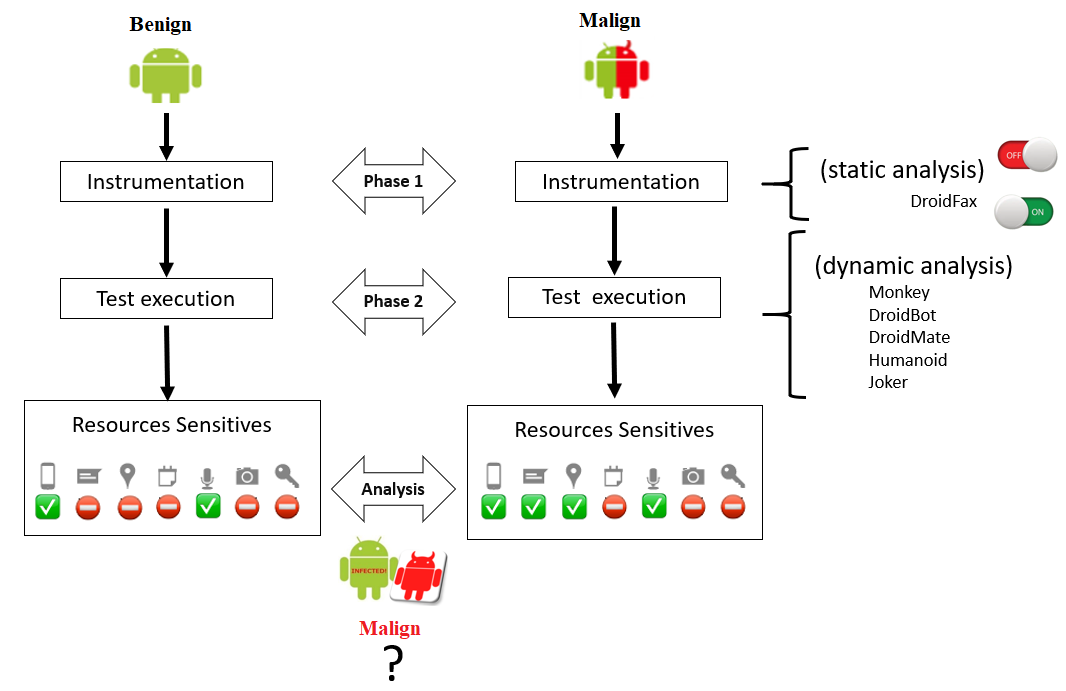
\includegraphics[width=0.75\textwidth]{images/setup3.png}}
   \label{Experiment setup}
   \caption{Experiment setup}
   \label{fig:setup}
 \end{figure}

\subsection{Second Study: Use of Taint Analysis for Malware Identification}\label{sec:set2}

In the second study 
we investigate whether or not a taint-based static analysis approach is also promising for
identifying malwares, given a version of an app that we can assume to be secure.
To this end, we leverage the FlowDroid
taint analysis algorithms for Android apps, at version 2.8, in order to identify dataflows
that might lead to the leakage of sensitive information. Our
goal here is to investigate if it is possible to detect malicious
behavior by means of identifying the \emph{divergent} source-sink paths that FlowDroid reveals after
analysing a benign and a malign versions of an Android app.

\subsubsection{Source-sink paths extraction}

FlowDroid takes as input an Android Application Package (APK file) and
a set of API methods marked either as {\bf source}
or {\bf sink} (or both). Source methods are those that access \emph{sensitive information} (e.g.,
a method that access the address book), while sink methods are those 
that \emph{might share information with external peers} (e.g., a method that
sends messages to a recipient). We rely on the source-sink definitions
of the FlowDroid implementation~\cite{arzt:pldi-2014,rasthofer-source-sink},
which involves a curate list of source and sink methods (including callbacks and
other Android API methods of interest).
FlowDroid then uses a \emph{context, flow, and field
sensitive analysis} to identify all dataflow paths from sources to sinks~\cite{arzt:pldi-2014}.

Source-sink paths extraction involve two steps (see Figure~\ref{fig:settings2}). In the first, we execute FlowDroid to mine the source-sink paths from a benign version of an app, and then enumerate a set (S1) with the 
possible dataflows between sources and sinks. All paths in S1 are considered secure for
our future analysis. In the second step we repeat the FlowDroid execution, though
considering the malicious APK version of the app.
This leads to a second set (S2) of source-sink paths.

\subsubsection{Source-sink paths analysis}

For our analysis it is important to note that not all source-sink paths are malicious, and then we
follow a specific methodology to identify malware in our work: we raise a warning (a \emph{hit}) whenever
FlowDroid finds an additional source-sink path in the malicious version of an app, which
has not been identified when analysing the benign version. For this end, we compute the difference (S3) between the sets S2 and S1 (i.e., $S3 = S2 \setminus S1$), in order to reveal the existence of additional paths in the malicious version (third step). If the set S3 is not empty, we conclude that FlowDroid
identified the malware.

We use two metrics in this second study:
the total number of malicious apps FlowDroid is able to find and the execution time for running the taint analysis algorithm for each app. Moreover, in this second study we use the same dataset of $96$ pairs of Android apps (B/M) used in the First study. Our second study will lead to discover what is the capacity of malware detection of taint analysis algorithms compared to mining sandbox approach, and its potential to complement dynamic analysis for mining sandboxes, thus answering our last research question (RQ3).


\begin{figure}
  \centering{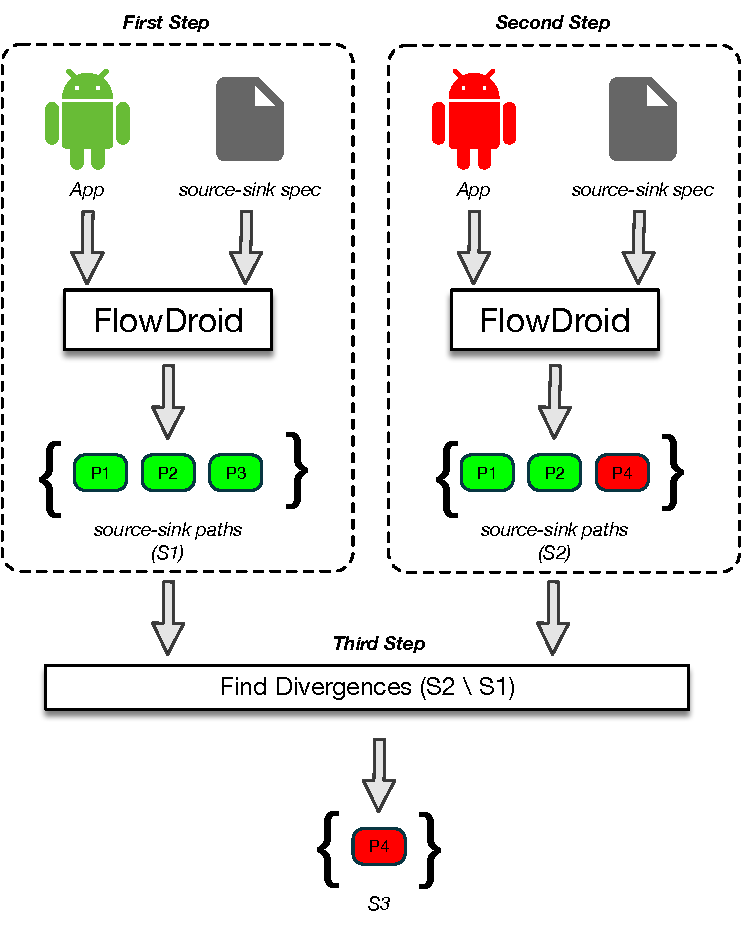
\includegraphics[scale=0.4]{images/second-study-settings.pdf}}
  \caption{Overview of our approach in the second study.}
  \label{fig:settings2}
\end{figure}








\section{Results and discussion}

In this section we detail the findings of our study. We first present the results of each study
in Section~\ref{sec:res-fs} and Section~\ref{sec:res-ss}. In Section~\ref{sec:discussion} we summarize the
implications of our study. 

\subsection{Result of the first study: A non-exact replication}\label{sec:res-fs}

Our first study performed a non-exact replication of Bao et al work.
Our study differs from the original because here we isolated the effect
of the DroidFax static analysis algorithms in the performance to
identify malicious apps using the test case generation tools for
mining sandboxes. In addition, we discarded six pairs of
Android apps we were not able to instrument---out of the $102$ pairs used in the \original work.
\rb{All of this following information should be detailed in
the study settings, and not repeated here if it is already there.} {\color{red}We also introduced a recent test generator tool, that has not been considered at previous work, Humanoid, and different from the original study, we expand the execution time of each test generation tool, executing each app at each tool for three minutes, while the original study executed for just one minute. The purpose of this time expansion is to check if the test generation tool code coverage results are consistent with Bao et al. results.}

As discussed in the previous section, we first executed the analysis using the DroidXP benchmark with its default configuration. After that, we executed the analysis again though disabling the DroidFax static analysis algorithm, so that we could better estimate the performance of the dynamic analysis tools for mining Android sandboxes. Table~\ref{tab:fs} summarizes the results of the execution. The columns Exec. (I) and Exec. (II) 
show the number of malwares identified when executing each tool (I) with the
support of the DroidFax static analysis algorithms and (II) without the support
of DroidFax static analysis algorithms. The Improvement column shows the impact
(in percentage) of DroidFax static analysis algorithms in the results.
In the previous work~\cite{}, the authors do not present a
discussion about the influence of DroidFax in the results, even
though here we report that this difference is in the
range from 23.94\% (Monkey) to 69.39\% (Humanoid)---discarding our
\joke tool for which DroidFax improves its performance in 100\% (as expected).
Next we discuss the result of each individual test generation tool. 

\begin{table}[ht]
  \caption{Summary of the results of the first study. }
  \centering
  \begin{small}
 \begin{tabular}{lrrr}
   \toprule
   Tool & Exec. (I) & Exec. (II) & Improvement (\%) \\   \midrule
  Monkey &  71 &  54 & 23.94 \\ 
  DroidMate &  64 &  48 & 25.00 \\ 
  DroidBot &  68 &  54 & 20.59 \\ 
  Humanoid &  49 &  15 & 69.39 \\ 
  \joke &  42 &   0 & 100.00 \\ 
 \bottomrule
 \end{tabular}
 \end{small}
 \label{tab:fs}
\end{table}


\subsubsection*{Monkey} sandbox for the first execution (Exec. (I)) detected more apps with malicious behavior than any other tool considered in our study (71 out of the 96 pairs of Android apps). Contrasting, in the original study, Monkey got the third-best performance, detecting 48 malwares within the 102 pairs (47.05\%). This difference might be due to the Monkey randomly strategy for test case generation. \rb{I am not convinced that the other tools do not employ any randomness.} For our second execution (Exec. (II)), there is a reduction of 23.94\% in the Monkey's performance, totaling 54 malware detected---which matches the performance of DroidBot for Exec. (II). \rb{Considering only one run for each configuration, that is Exec. (I) and Exec. (II), we cannot assure that the difference is due to disabling the DroidFax static analysis algorithms.}


\subsubsection*{DroidBot} in the first execution (Exec. (I)) its resulting sandbox detected a total of 68 malware among $96$ pairs analyzed (70.83\%). Interesting, this is the same performance of the original study---although the original study analyzed $102$ pairs of Android apps. Also, in the original study, DroidBot was the test case generation tool whose resulting sandbox detected the largest number of malicious apps. However, in our second execution (Exec. (II)), its performance decreased in 20.58 \%. \rb{Not sure if the following sentence is right.} Despite this reduction, it achieved the largest number of malicious apps detected in the second execution.

\subsubsection*{DroidMate} in the first execution led to a sandbox that detected 64 apps with malicious behavior (66.66\%). Contrasting, in the original study DroidMate detected 54 among 102 (52.94\%). A possible explanation for this difference is that here we use the more recent version of DroidMate. In the second execution, without the DroidFax static analysis algorithms, the resulting sandbox's performance drops by 25\%, being able to detect 48 out of the 96 pairs of Android apps. 


\subsubsection*{Humanoid} presented the worse performance, even though a previous
work~\cite{DBLP:conf/kbse/LiY0C19} shows that it presents the highest lines coverage in comparison to Monkey, DroidBot, and DroidMate. In the first execution (Exec. (I)), the resulting Humanoid sandbox identified 49 malwares in our dataset (51.04\%). Since Bao et al. did not explored Humanoid in their study, we do not have a baseline for comparison. Regarding the second execution, without static analysis, Humanoid was the most affected by disabling the DroidFax static analysis algorithm, losing 69.38\% of its effectiveness, and being able to detect just 15 malwares.

\subsubsection*{\joke} is our fake test case generation tool that we use to help us understand the performance of the DroidFax static analysis algorithm for mining sandboxes. We integrated \joke into the DroidXP benchmark as an additional test generation tool that does not run the Android apps during the benchmark execution. As a result, the analysis using \joke reveals the performance of DroidFax static analysis algorithms only. For the first execution, with the DroidFax static algorithms enabled, even though \joke does not execute the Android apps, its resulting sandbox detected 43.75\% of the malwares. For the second execution, that is, disabling the DroidFax static analysis algorithm, the resulting \joke sandbox was unable to detect any malware. This result was expected, since \joke does not analyze the Android apps during the benchmark execution.

\begin{finding}
  Integrating the dynamic analysis tools
  with the DroidFax static analysis algorithms
  improves substantially the performance
  of the resulting Android sandboxes for
  detecting malicious behavior. 
\end{finding}
 
The Venn-diagram of Figure~\ref{fig:venn-plot1}
summarizes how the tools can complement each other.
Note in the diagram that 47 malwares have been detected by all sandboxes generated in the first execution (with the DroidFax static analysis algorithms), out of the 77 identified by at least one sandbox. In addition, the DroidBot sandbox did not detect any malware that had not been detected by the other tools. Differently, the Monkey's sandbox detected five malwares that had not been detected by any other sandbox, DroidBot sandbox detected four malwares that had not been detected by any other sandbox, and Humanoid detected one malware that had not been detected by any other sandbox. Contrasting with the Bao et al. work~\cite{DBLP:conf/wcre/BaoLL18},
our results suggest that using DroidBot in combination with Monkey, DroidMate, and Humanoid does not improve the general performance of an integrated environment for mining
Android sandboxes.  

\begin{finding}
  Our results suggest that one might benefit from using  an integrated
  environment that combines Monkey, DroidMate, and Humanoid to
  mine Android sandboxes. Introducing the DroidBot 
  tool does not improve the results.
\end{finding}


\begin{figure}[htb]
  \centering{
  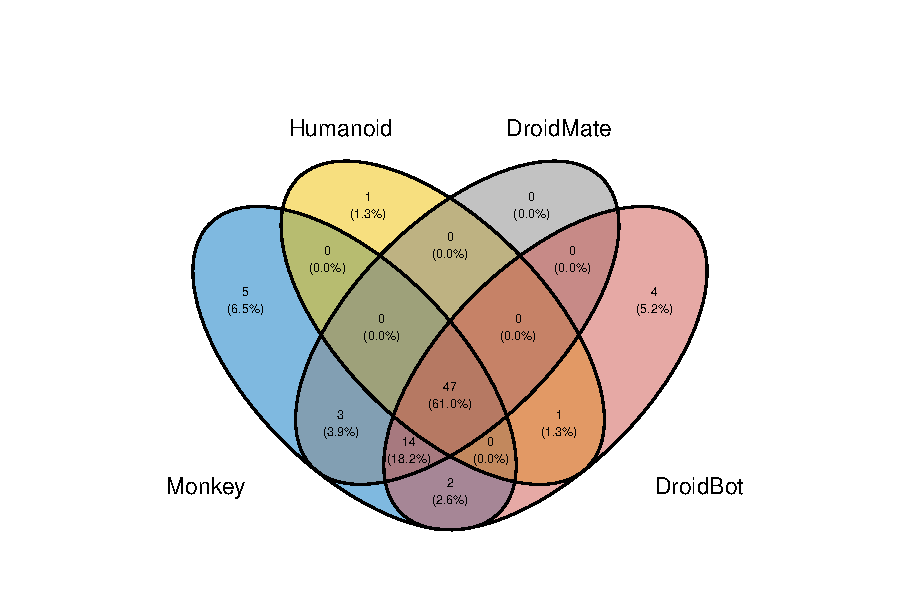
\includegraphics[trim=60 20 0 50,scale=0.7]{images/venn-plot-1.pdf}}
  \caption{Venn Diagram highlighting how the sandboxes from the tools can
    complement each other.}
  \label{fig:venn-plot1}
\end{figure}


Altogether, ignoring the \joke tool, our study reveals that from 51.04\% (Humanoid)
to 73.95\% (Monkey) of the malicious apps investigated in our study can be
detected using the sandboxes generated after running the test case tools with the support of DroidFax static analysis algorithms. Besides that, in the first execution, none of the resulting sandboxes could detect 19 malwares in our dataset (19.79\%). According to the Euphony tool~\cite{hurier2017euphony}, 13 of these 19 malwares are \emph{adwares}, three are \emph{trojans}, two are PUPs (\emph{Potentially Unwanted Program}), and one is an \emph{exploit}. \rb{In what follows we present some characteristics of malwares that had not been detected by the sandboxes.}

\rb{This is an interesting place to present the details of two or three malwares in this set of 19 malwares that had not been detected by any tool. I think Thales could work on this, since he has helped Handrick to dissect the malwares.}



\subsection{Result of the second study: Tainted analysis algorithms.}\label{sec:res-ss}

In this second study we used a tainted analysis approach to mine differences between the benign and malicious versions of each of the 96 Android apps in our dataset. To this end we leverage the FlowDroid tool, which tracks how sensitive information flows through the apps using tainted analysis algorithms. Regarding accuracy, the tainted analysis approach detected 58 out of the 96 pairs in our dataset (60,42\%), that is, the FlowDroid approach leads to a better performance than any sandbox originated in the second execution of the dynamic analysis tools (without the DroidFax static analysis algorithms).

\begin{finding}
  The performance of FlowDroid to identify malicious behavior
  using our approach is superior than the performance of the
  mining sandbox approach supported by dynamic analysis only---without
  the DroidFax static analysis algorithms.
\end{finding}

Additionally, we investigate if we could benefit from combining
the results from FlowDroid and DroidFax. Figure~\ref{}
shows the results.
Considering the static analysis provided by DroidFax and FlowDroid, our results showed that both were able to detect 33 pairs in common (34.37\%), and there were 29 pairs that both were not able to detect (30.20\%). We also realized that just 9 pairs were detected by DroidFax and do not by FlowDroid, while 25 pairs were detected by FlowDroid, and do not by DroidFax, evincing a better accuracy of tainted analysis algorithm.


The first results show that with tainted analysis, we had an analysis processing cost of 32.08 seconds per app pair on average, totaling a processing time of 52 minutes to analyze all the pairs. The processing time depends on the size of the app, and the pair that took the fastest time analyzed in 3 seconds and the longest 437 seconds. 


Table \ref{tab:comparison} compile the results of this comparison.

\begin{table}[htb]
\centering
\begin{tabular}{lcc}\toprule

Detected by  & Malwares detected & \%   \\ 
(DroidFax/FlowDroid) & (Among 96 pair) & \\ \midrule
Both tools & 33 & 34.37\%  \\
Just DroidFax & 9 &  \\
Just FlowDroid & 25 &  \\
None & 29 & 30.20\% \\\midrule
 
\multicolumn{1}{r}{Total} &   96 \\ \bottomrule
\end{tabular} 
\caption{Comparison between DroidFax and FlowDroid algorithms}
\label{tab:comparison}
\end{table}


Furthermore, we can highlight that among 19 pair apps that at first study, were not detected by the sandboxes constructed by test generation tool, and static analysis DroidFax miner, 4 were detected by FlowDroid; P35, P38, P56, and P94, therefore exposing better accuracy of the tainted analysis algorithms. Among these 4 pairs detected, 2 were trojans, 1 was the exploit, and 1 was adware.


\subsection{Discussion}\label{sec:discussion}

First we find that static analysis summaries had impact in the Bao et al. study. It was responsible for improving the results of the tools by 47.78\% than its executions alone, answering our first research question (RQ1). Second, Table \ref{tab:malwareWithout} summarizes our findings addressing the second research question (RQ2). We realized that disregarding the static analysis algorithms, and discarding Joke tool, among the tools analyzed in your study, Humanoid had the biggest performance drop, and the least affected was DroidBot, proving be the tool with better effective performance, in terms of the number of detected malware. Finally, we answered our last research question (RQ3) when we leverage sandboxes, complementing the dynamic analysis provided by test generation tool with tainted analysis algorithms. Our experiment highlight that 69.79\%-81.25\% of malware in dataset can be now uncovered by the complement of tainted analysis algorithms, evidencing that 
sandboxes can be further boosted when coupled with new static analysis techniques. We found that the number of identified malicious apps detected is increased for all cases, achieving at the best case, 81.25\% with Monkey, a better performance than all five tools explored at Bao et al., even when they combined all the tools together at theirs work 75.49\%. Table \ref{tab:tanted} display the increase of all tools explored at our research.

\begin{table}[ht]
\centering
\begin{tabular}{lccc}\toprule
 Test Generation & FlowDroid & Total & \%\\
 Tool & Increase  &  & \\ \midrule
 Monkey & 7 & 78 & 81.25\\
 DroidMate & 10 &  74 & 77.08 \\
 Humanoid & 20 & 69 & 71.87  \\
 Joke & 25 & 67 & 69.79 \\
 DroidBot & 9 & 77 & 80.20  \\\midrule
 
\end{tabular} 
\caption{Malwares detected in 96 pair (B/M) increased by Tainted analysis Algorithms}
\label{tab:tanted}
\end{table}

%%here we also have to write about the intersection between droidfax and tainted analysis now, and about what 1 reveled and other dont, and otherwise. 


%Here we can write about MOTIVATION EXAMPLES.

\section{Flowdroid for static analysis}
\section{Threats and future works}

Due to the randomization behavior presented by each chosen tool, we should not validate the results of this experiment without considering the presence of random events in the execution. To mitigate this, we have used a configuration of the benchmark DroidXP tool that runs multiple times each test and computes the average result from those executions. So, the comparison between the results of this experiment and the experiment presented by Bao et al. could be more precise.
Beyond that, we tested only 96 of the original 102 pairs of apps in this experiment because the benchmark could not execute those six pairs of apps due to crashes in the Android emulator. This difference threatens the validity of the comparison between the Bao et al.'s experiment and ours.
As future work, we plan to investigate other promising tools to enhance our data from previous executions. We will use the benchmark to test tools like Sapienz (a search-based test generation tool) \cite{DBLP:conf/issta/MaoHJ16} and Dynodroid (an input generation system for Android apps) \cite{DBLP:conf/sigsoft/MachiryTN13}. And we will search for other great tools used by academia and by the industry to be tested by the benchmark DroidXP.
Also, we will execute each of the tools used in this experiment without the benchmark. And, we will compare these results with this experiment's results. This comparison will be valuable in the pursuit of one of this study's goals, which was to analyze what impact the benchmark droidXP has on its results. 

\section{conclusion}

%\balance 
\bibliographystyle{IEEEtran}
\bibliography{ref}

\end{document}
